\section{Introduction}\label{sec:intro}
%Compared to traditional feature phones which are capable of voice calls and text messages,
%%
%smartphones bring many more applications including, but not limited to, email checking, web browsing, online shopping, game playing, music listening, video shooting, and GPS navigation.
%%
%%enable users to check their email, browse the web, post updates to social media sites, shop online, play games, listen to music,  shoot photos, and so on.
%%
%%can provide users with much more services such as email checking, web browsing, game playing, music listening, social chatting, video shooting, and so on. 
%%
%%
%With such extensive capabilities, smartphones have become ubiquitous and all-pervasive.
%%
%Indeed, the total number of smartphone users worldwide is over 3 billion this year - nearly 40\% of the human population, according to reports issued by several market-research firms~\cite{report2018newzoo,report2019forrester}. 

Smartphones have become one of the most popular devices in the last few years. According to Statista~\footnote{\url{https://www.statista.com/statistics/330695/number-of-smartphone-users-worldwide/}}, the current number of smartphone users in the world today is over 3 billion, and this means nearly 40\% of the world’s population owns a smartphone. 

In this thesis, however, we demonstrate how to turn smartphones to spy bugs which eavesdrop on everything played by smartphones' built-in speakers. Three billion smartphones? No, they are 3 billion spy-phones!
%
This dreadful attack, referred to as the \textit{{\attackName}} attack, is based on the fact that motion sensors (accelerometers and gyroscopes) can catch acoustic signals like a crude microphone. 
%
Thanks to smartphones' operating systems, accessing these sensors is effortless. 
For example,  Android
\footnote{\scriptsize iOS, Windows, and Blackberry OS have similar permission-based sensor management systems~\cite{sikder20176thsense}. In this work, we focus on Android.} 
automatically grants app permissions to motion sensors at installation time. In other words, any app installed in a smartphone can be a tool for attackers to eavesdrop covertly.
%iOS, Windows, and Blackberry OS have similar permission-based sensor management systems~\cite{sikder20176thsense}. In this work, we focus on Android.

%without notice. 
An example of attacking scenarios is illustrated in  Figure~\ref{fig:teaserpic}. A boy has a video call with his mom. He wants to buy a book online and he needs her mom’s credit information to place an order. Her mom’s voice is played by the loudspeaker on the smartphone and affects the readings by motion sensors. The attacker has access to the motion data and therefore can infer the credit card information.  
%

\begin{figure}
	\centering
	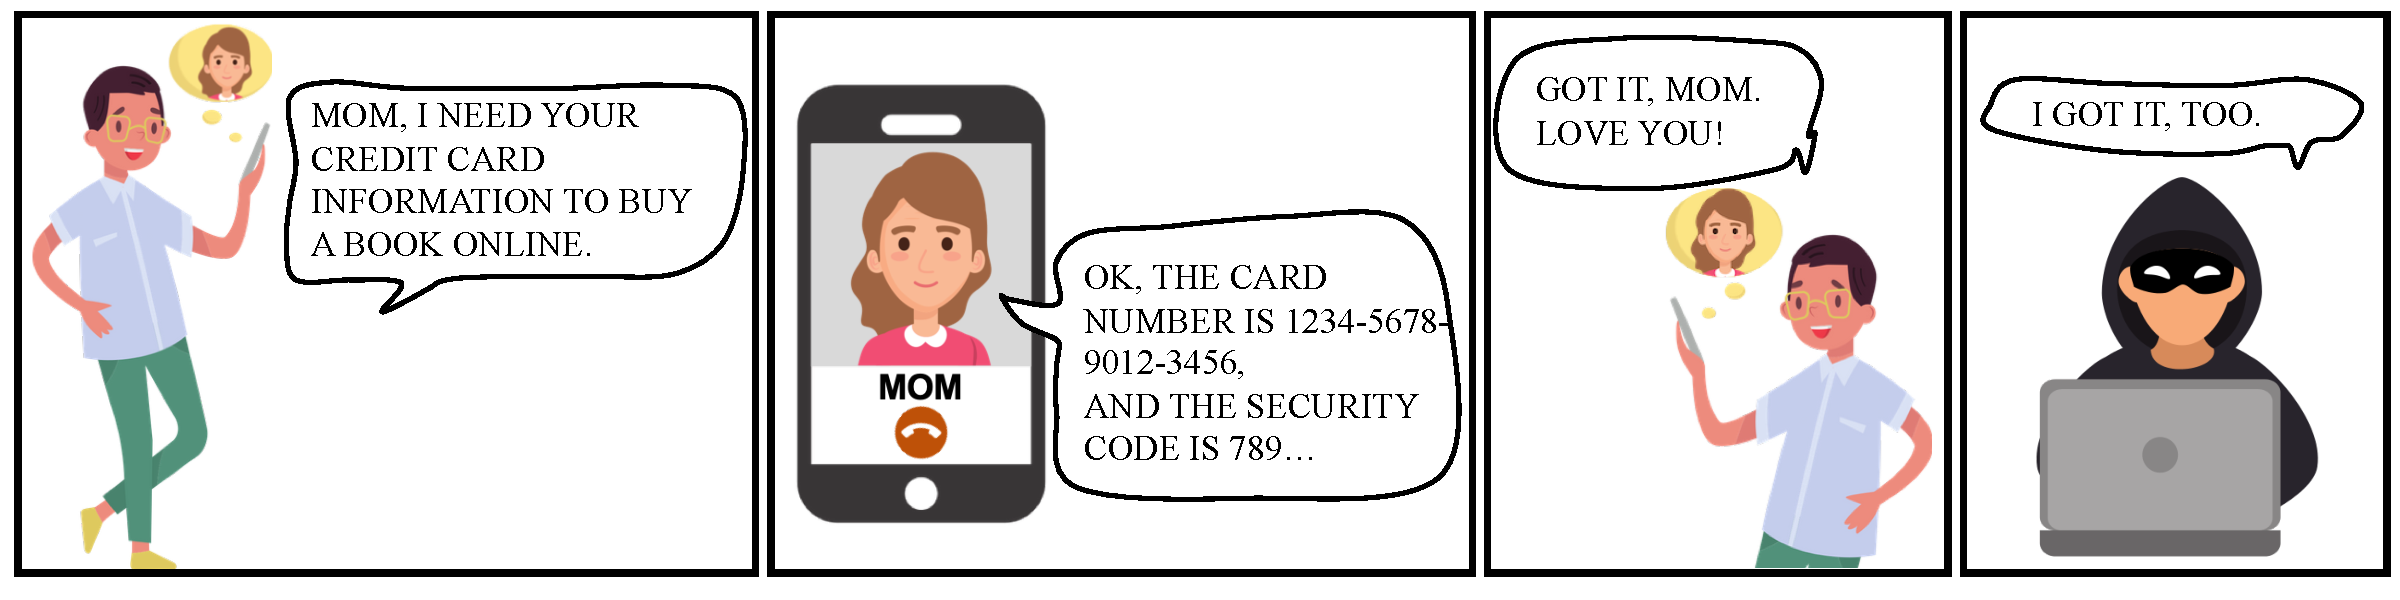
\includegraphics[width=\linewidth]{Figures/SpyPhone/teaserpic}
	\caption[Example of an Attacking Scenario.]{Example of an Attacking Scenario by {\spp}. A seemingly harmless application (a weather app for example) is installed on the phone, and it keeps accessing the motion sensors in the background. Attackers can infer acoustic signals from the under-sampled motion data. }
	\label{fig:teaserpic}
\end{figure}



In fact, there have been some recent studies about the side-channel leakage from acoustic signals to smartphones' motion sensor readings. Michalevsky et al.~\cite{michalevsky2014gyrophone} proposed \textit{Gyrophone} in 2014. To the best of our knowledge, they are the first to use smartphone gyroscopes as low-frequency microphones to listen to loudspeakers. Gyrophone can differentiate 11 digits with 65\% accuracy based on a 10 people dataset.
One year later, Zhang et al.~\cite{zhang2015accelword} proposed \textit{AccelWord}, which utilizes accelerometers to classify hotwords such as ``Okay Google'' or ``Hi Galaxy'' over other short phrases with 85\% accuracy. AccelWord is also tested over 10 people.


However, techniques proposed in neither Gyrophone nor AccelWord can be used to perform a {\attackName} attack. Because these systems are built upon a \textit{speaker-dependent} model, i.e. training dataset are labeled data from the target speakers. In the {\attackName} attack, attackers will not get \textit{labeled} motion data from the victim  ------ the attack system should be \textit{speaker-independent}.

In 2018, Anald and Saxena~\cite{anand2018speechless} reproduced the aforementioned works and overturned their conclusions. They argued that smartphone motion sensors can not be affected by the speech signals transmitted through the air, no matter the sound source is a loudspeaker or a live person. They reported that only when the speakers and the motion sensors sharing a surface,  the \textit{conductive vibrations} will affect motion sensors' readings. Except for this ``Loudspeaker-Same-Surface'' scenario, they studied 5 other  scenarios
\footnote{\scriptsize``Loudspeaker-Different-Surface'', ``Laptop-Same-Surface'', `` Phone-Different-Surface'', 		``Human-Normal'', and ``Human-Loud''.}  
and concluded that smartphone motion sensors only pose a limited threat to speech privacy.
%
However, they missed one important scenario,  the \textit{intra-device} scenario, where the speakers and motion sensors are inside the same smartphone. In 2019, they investigated this remaining scenario in an arXiv paper~\cite{anand2019spearphone} and their SpearPhone system recognizes 11 digits with an accuracy of 71\%.  However, their technique is still speaker-dependent, which means the original speech data of the target speaker must be collected ahead of time. Such a requirement is very hard to be fulfilled in practice.

In this thesis, we studied the side-channel attack in the intra-device scenario. This \textit{{\attackName}} attack, as we refer to it, is speaker-independent.


\begin{table}[h]
	\caption{Maximum Sampling Rate of Smartphone Sensors}
	%	\footnote{Some part of the data is from~\cite{matyunin2018zero}, others are tested }
	\label{tab:sample}
	\centering
	
	%	\resizebox{\columnwidth}{!}{
	\begin{tabular}{cccc} %{lp{2cm}p{2cm}}
		\toprule		
		Device & \makecell{Release \\Year} & \makecell{Speakers' \\ Sampling Rate} & \makecell{Motion Sensors' \\ Sampling Rate
			\footnotemark} \\
		\midrule
		Samsung Galaxy S8 & 2017 & 192,000 Hz & 500 Hz\\
		Samsung Galaxy S7 & 2016 & 192,000 Hz & 500 Hz\\		
		Google Nexus 6P & 2015 & 48,000 Hz & 400 Hz\\
		LG Nexus 4 & 2012 & 48,000 Hz& 200 Hz\\
		\bottomrule
	\end{tabular}
	%}
\end{table}



\footnotetext{\scriptsize Data is partially from~\cite{matyunin2018zero} and partially by calling the \texttt{getMinDelay()} function of \texttt{android.hardware.Sensor} class.}

The main challenges in designing such a system are:
 \begin{itemize}
 	\item  The motion sensor readings are affected by at least four types of signal sources: sensor intrinsic errors, movement of the smartphone, acoustic vibrations from built-in speakers, acoustic vibrations from the air or other sound sources. An efficient filter is needed since only the acoustic vibrations from built-in speakers is the signal of interest.
 	
 	\item As shown in Table~\ref{tab:sample}, compared to the sampling rate of smartphones' built-in speakers which can reach 192 kHz, the sampling rate of motion sensors is 200-500 Hz. With such low frequency, human ears are no longer able to retrieve the original information, neither do state-of-the-art speech recognition systems~\cite{michalevsky2014gyrophone}.
 	
 	\item As illustrated in Figure~\ref{fig:depend}, the system should be speaker-independent. Prior works such as  Gyrophone~\cite{michalevsky2014gyrophone} and AccelWord~\cite{zhang2015accelword} can only achieve the claimed accuracy (65\% for 11 classes and 85\% for 3 classes) in the speaker-dependent setting. When Gyrophone uses a speaker-independent setting to identify digits, the
 	accuracy is only 26\%. This indicates that building a speaker-independent system is much more challenging than a speaker-dependent one.
 
 \end{itemize}



Despite these challenges, the {\systemName} system is able to learn a variety of critical information from smartphone users, such as user activity, speaker gender/identity, and speech content (as elaborated in Section~\ref{sec:threat}). 
These achievements are largely credited to the compressed sensing theories which allow recovering certain signals from fewer samples than required in Nyquist paradigm (as elaborated in Section~\ref{sec:background}); and the machine learning techniques named Bi-directional Long Short-Term Memory (Bi-LSTM) network, which is a special variant of recurrent neural networks. 




\begin{landscape}
	\begin{figure*}[h]%
		\centering
		\begin{minipage}[c]{.45\linewidth}
				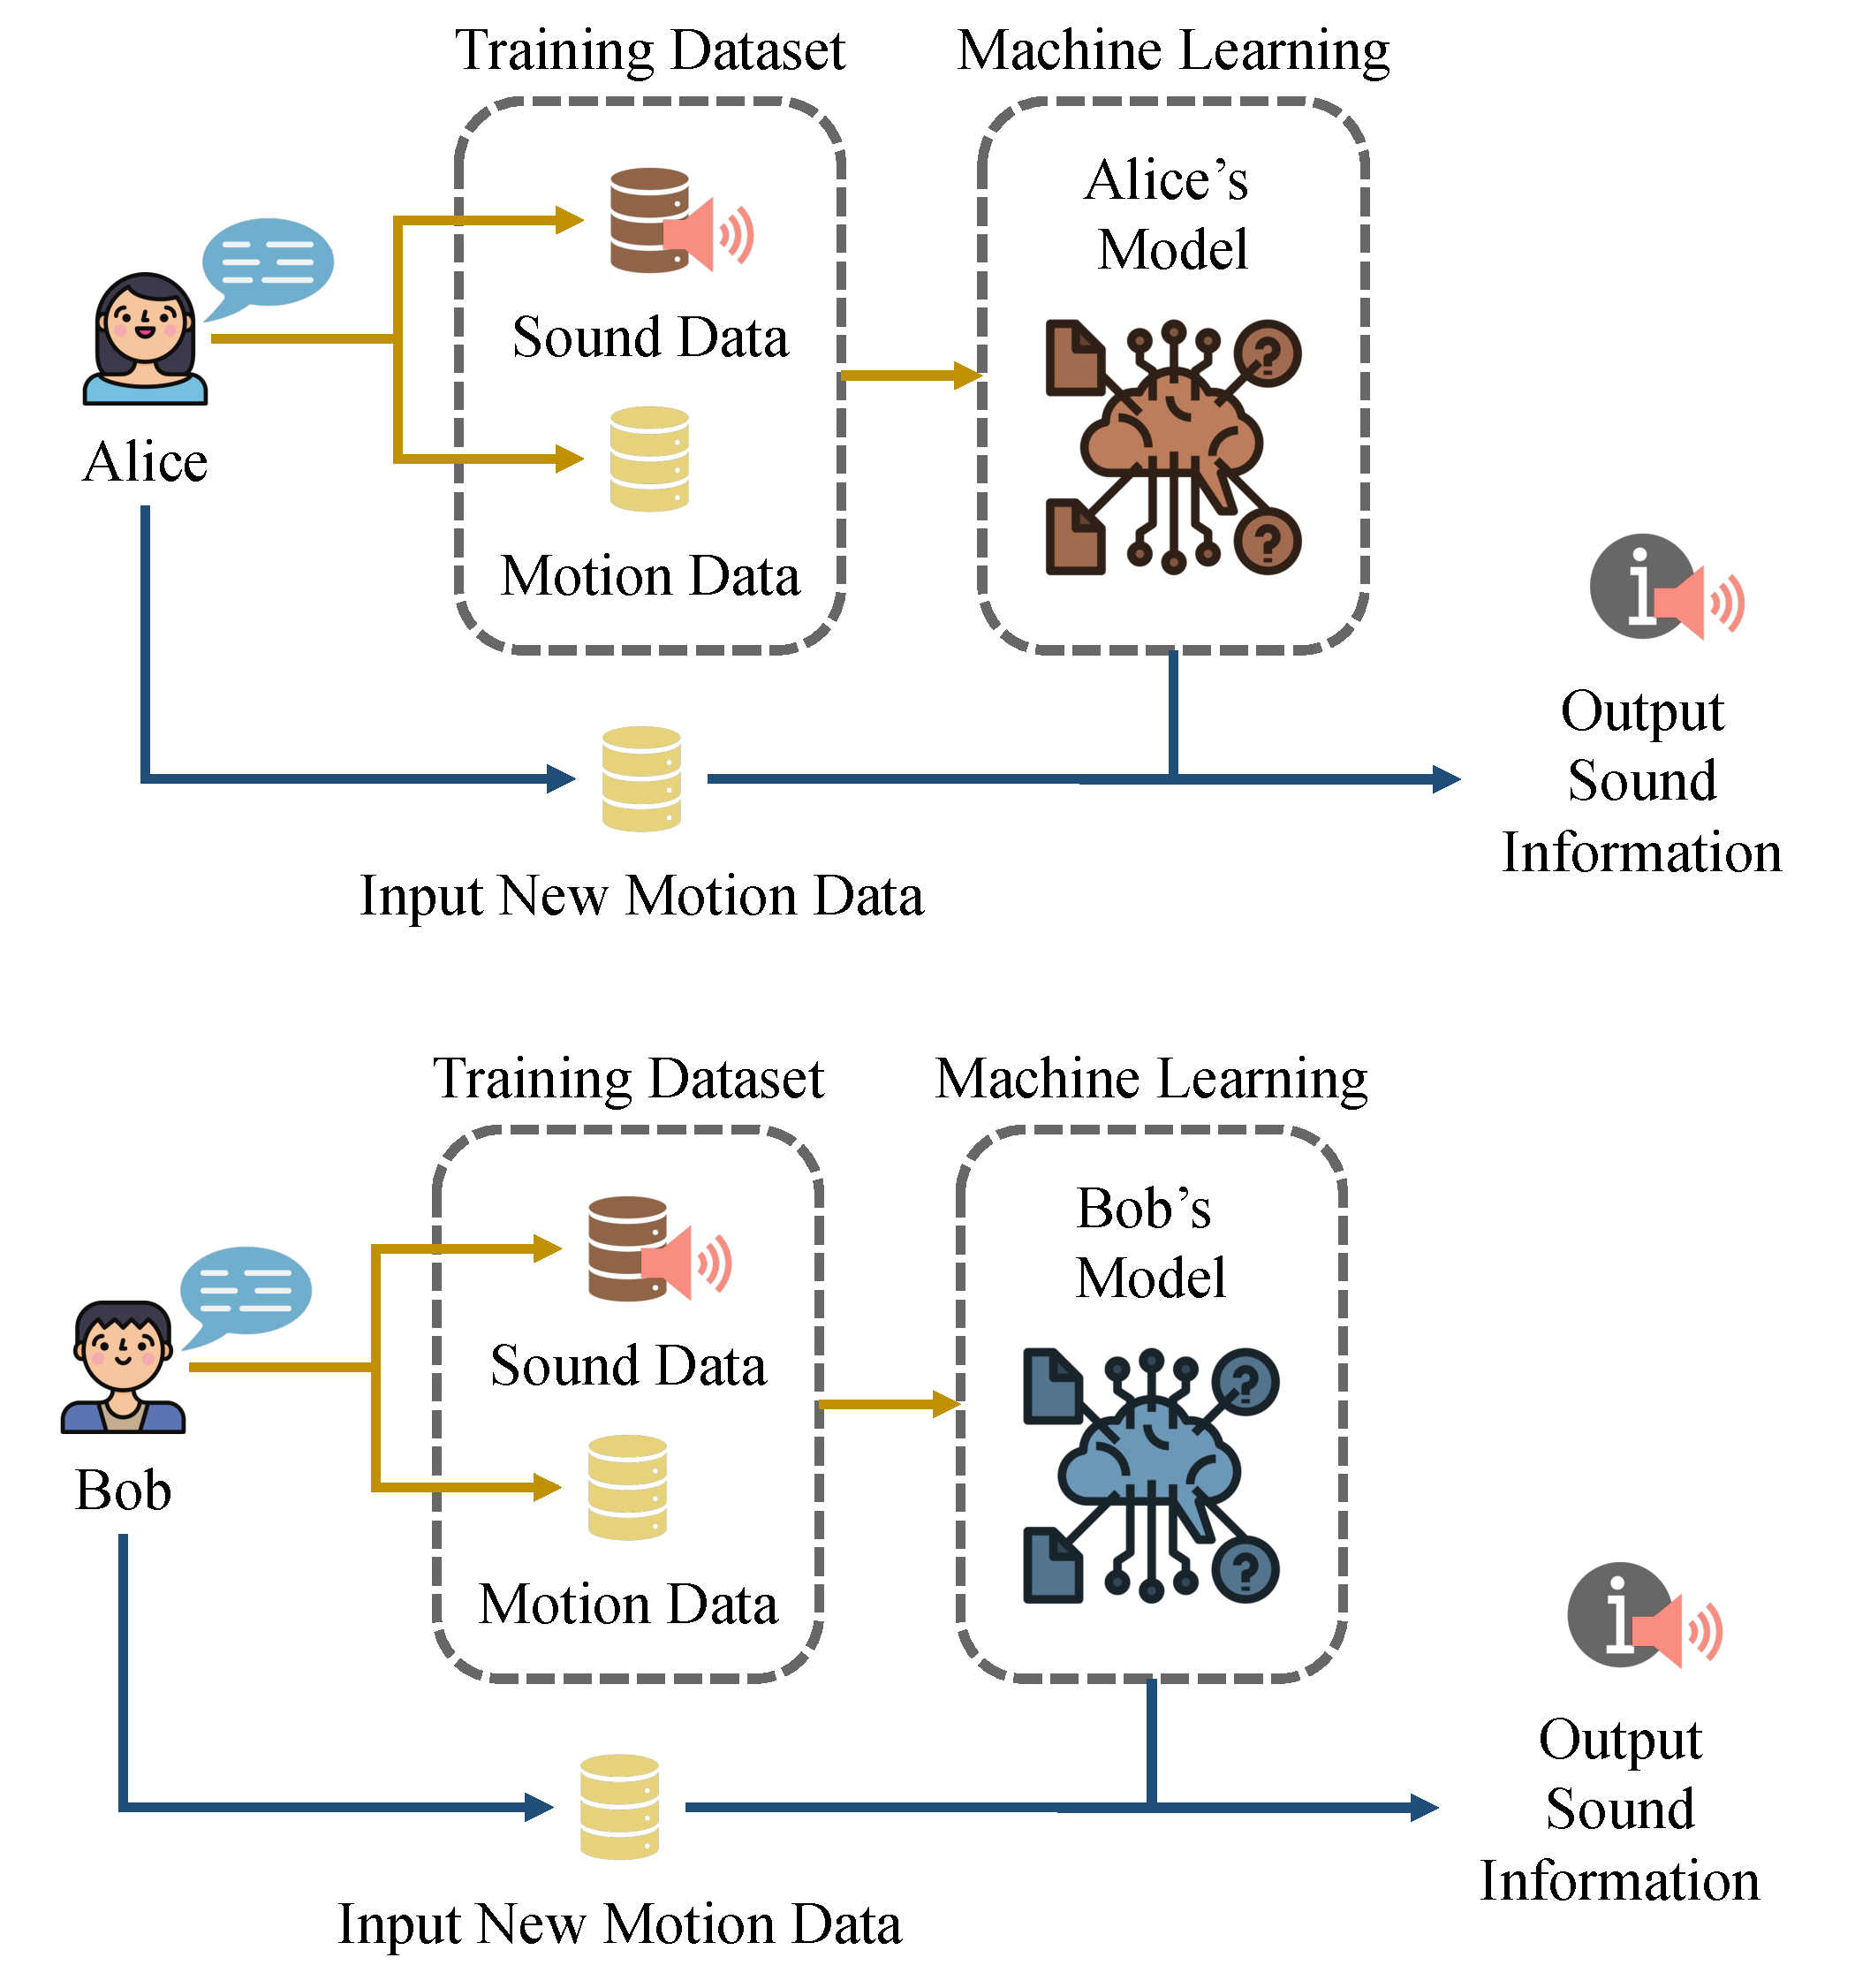
\includegraphics[width=\textwidth]{speakerDependent}
				\subcaption{Speaker-Dependent: the target speaker's training data is required. After machine learning procedures, the trained models  for different speakers are different.}
		\end{minipage}
		\begin{minipage}[t]{.05\textwidth}
			\qquad
		\end{minipage}
		\begin{minipage}[c]{.45\linewidth}
				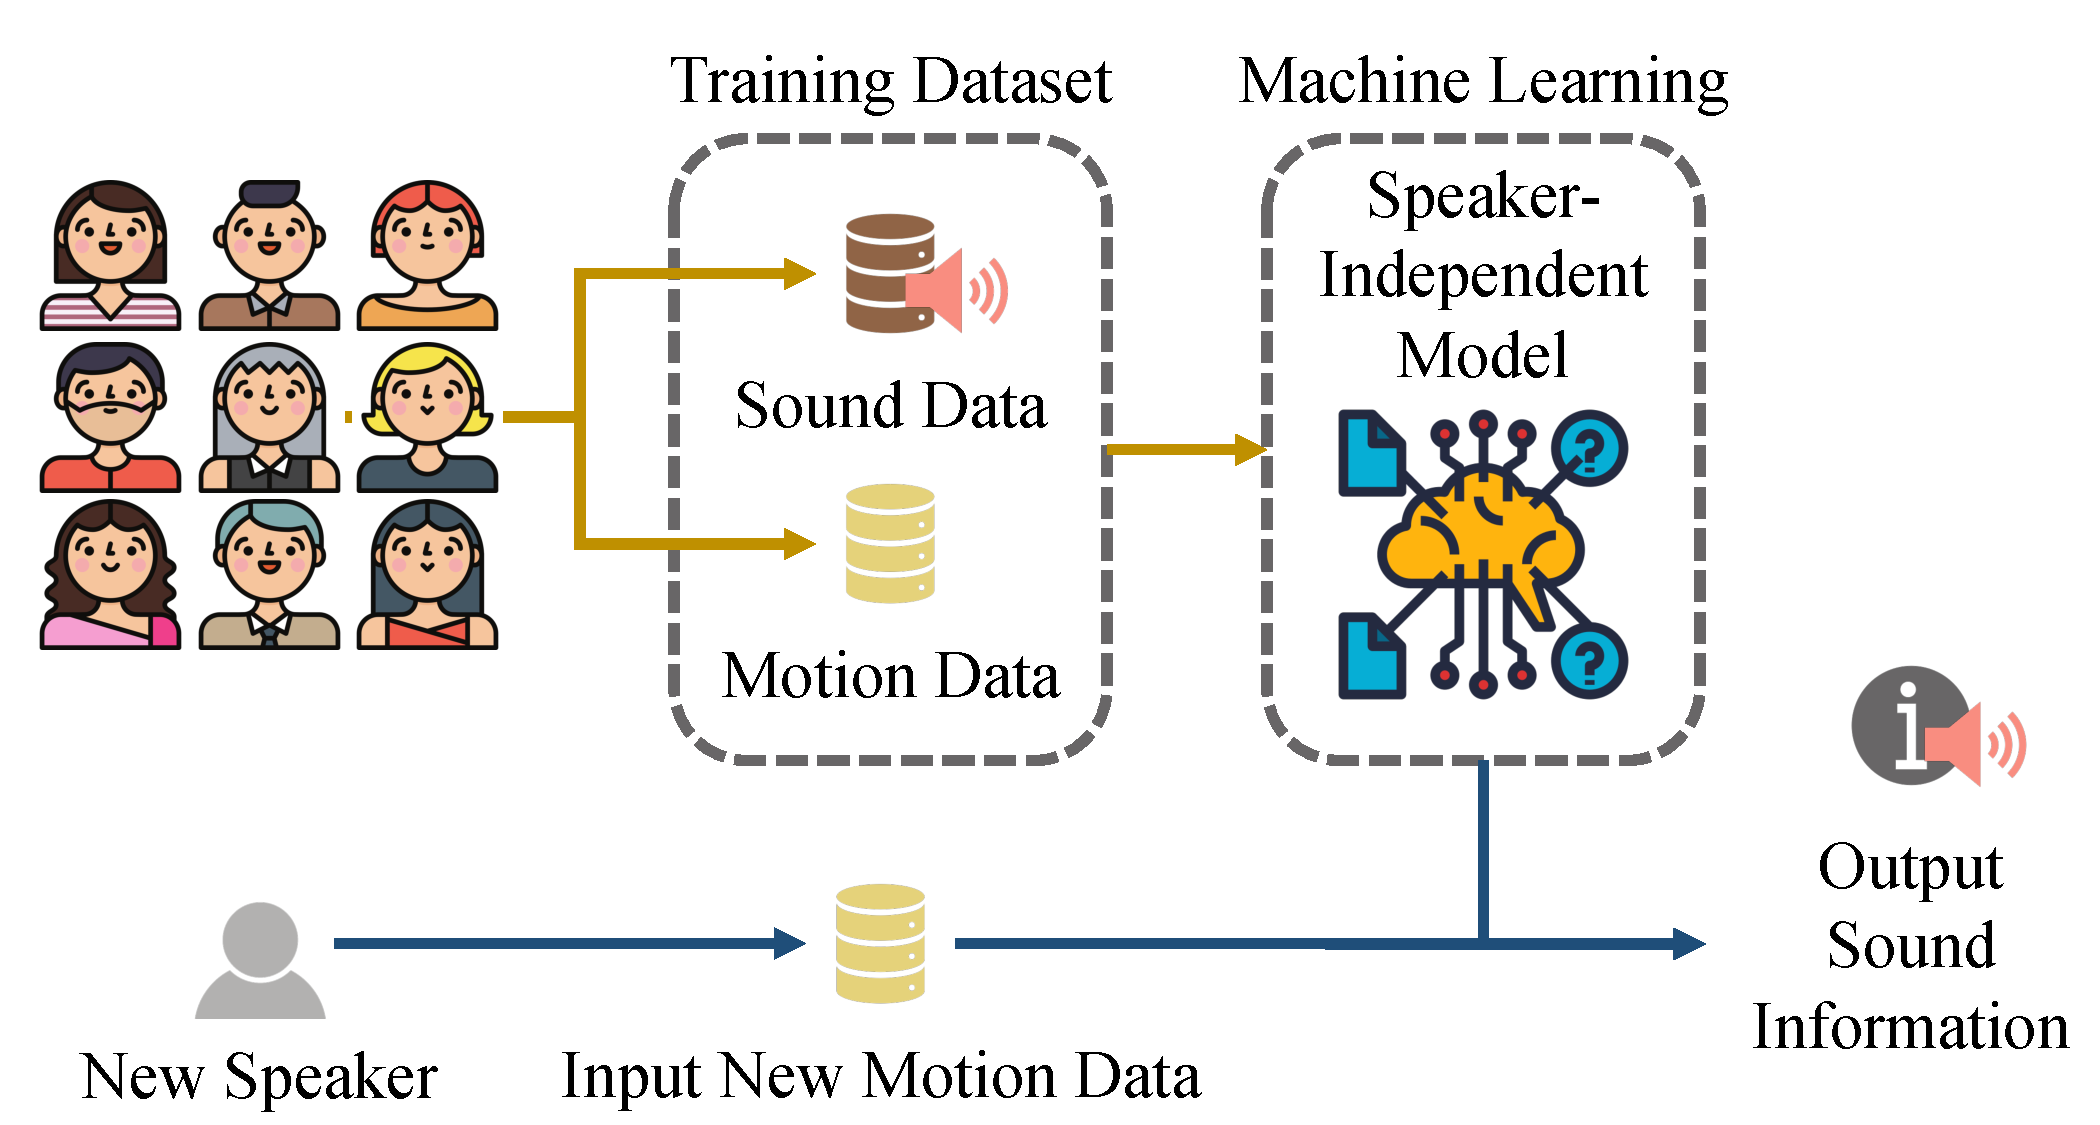
\includegraphics[width=\textwidth]{speakerIndependent}
				\subcaption{Speaker-Independent: the model is trained on a group of speakers, and can be used to predict brand new speakers.}
		\end{minipage}
		\caption{{\attackName} Attack Should be Speaker-Independent.} \label{fig:depend}
	\end{figure*}
\end{landscape}

In summary, our main contributions are as follows:
\begin{itemize}
	\item 
	We uncover a new stealth attack named the {\attackName} attack that eavesdrops on smartphones' built-in speakers by the intra-device motion sensors. Existing techniques in Gyrophone~\cite{michalevsky2014gyrophone} and AccelWord~\cite{zhang2015accelword} cannot be used for the {\attackName}  attack because their systems are speaker-dependent, which require the training speech data from the victim. The {\attackName}  attack, however, removes this requirement and thus is more dangerous and harmful.
	
	\item 
	To the best of our knowledge, we are the first to apply compressed sensing theories in the audio-to-motion side-channel data so as to bridge the gap between sampling rates. This is the core technique we used to achieve the speaker-independence of the attacking system.
	
	
	\item 
	We design the {\systemName} system and validate its feasibility on learning user activity, speaker gender/identity, and speech content.  {\systemName} system can achieve higher accuracy than existing works. Besides, we have studied how different internal parameters (used in algorithms) and external parameters (properties of input data) affect the  performance of this system.
	
\end{itemize}
